\section{Multiple issue}
Il Multiple Issue è la capacità fondamentale delle moderne CPU superscalari di prelevare, decodificare ed accettare più istruzioni contemporaneamente nello stesso ciclo di clock. Per sostenere questo parallelismo, l'architettura interna necessita di un potenziamento significativo: bisogna allargare il bus degli operandi per gestire il trasferimento simultaneo di dati e potenziare la logica di emissione e scheduling delle istruzioni. Il processo è estremamente rapido e prevede l'assegnazione preventiva delle risorse necessarie e una meticolosa analisi delle dipendenze tra tutte le istruzioni candidate all'emissione, al fine di evitare conflitti di dati (RAW, WAW, WAR). L'implementazione hardware è complessa perché le tabelle di stato interne che tracciano l'uso delle risorse (come i registri e le unità funzionali) devono essere aggiornate in parallelo per l'intero bundle di istruzioni e completare il tutto in un solo ciclo di clock. Inoltre, il controllo delle dipendenze tra più istruzioni richiede un numero massivo di operazioni di confronto eseguite in parallelo, generando un notevole overhead logico. È difficile superare le quattro istruzioni emesse per ciclo perché l'aumento della complessità logica e il conseguente ritardo sul clock spesso superano i guadagni di prestazione. Questa soglia è critica anche perché la speculazione (l'esecuzione predittiva) deve continuare a funzionare in modo efficiente; gestire troppe istruzioni speculative in contemporanea aumenta drasticamente il costo di un errore di predizione. Per migliorare l'efficienza, una strategia comune è separare le istruzioni intere da quelle in virgola mobile, permettendo un scheduling più flessibile e l'uso di unità funzionali dedicate. Altre unità di supporto giocano un ruolo cruciale: un'unità di prelievo (fetch) efficiente con un'unità branch integrata per la predizione dei salti e la disponibilità di più linee di cache L1 aiutano a mantenere il flusso di dati e istruzioni. Le sfide aggiuntive includono l'elevato consumo energetico derivante dall'attivazione parallela di molteplici componenti, la penalizzazione causata dai mancati accessi alla cache che possono bloccare interi bundle di istruzioni, e la complessità di gestire più istruzioni di salto speculative nello stesso ciclo di emissione.

\begin{figure}[ht]
    \centering
    \setlength{\fboxrule}{0.5pt} % spessore sottile
    \setlength{\fboxsep}{0pt}    % senza spazio interno
    \fbox{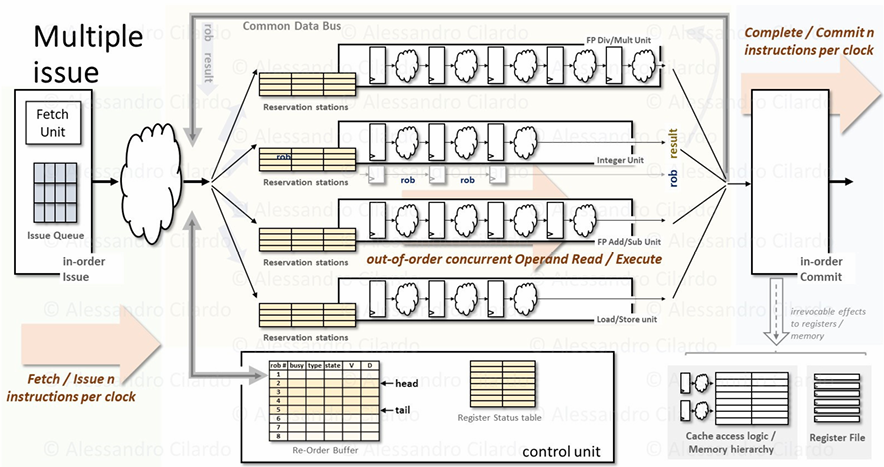
\includegraphics[width=0.75\textwidth]{fig/chapter_2/multiple_issue.png}}
\end{figure}

\noindent Il parallelismo interno è possibile grazie alle tecniche hardware e software fin qui presentate; viene demandata al programmatore, tramite il supporto hardware, l'espressione di ulteriore parallelismo.